\documentclass[a4paper,11pt]{article}
\usepackage[czech]{babel}
\usepackage[a4paper, total={170mm, 240mm}, top=2cm, left=2cm]{geometry}
\usepackage[utf8]{inputenc}
\usepackage[T1]{fontenc}
\usepackage{times}
\usepackage[hidelinks]{hyperref}
\usepackage{graphicx}
\usepackage{booktabs}
\usepackage{epstopdf}
\usepackage[htt]{hyphenat}
\usepackage{amsmath}
\usepackage{float}
\usepackage{indentfirst}
\usepackage{array}
\usepackage{enumitem}
\usepackage{bm}

\begin{document}
\begin{center}
\Huge
\textsc{Vysoké učení technické v~Brně\\
}Fakulta informačních technologií\\
\vspace{\stretch{0.382}}
\Huge Technická zpráva \\
\LARGE  Aplikace ovládaná dvojicí rotačních enkodérů \\
\vspace{\stretch{0.309}}

\Large 

\vspace{\stretch{0.309}}

\end{center}
{\Large \today \hfill
\begin{tabular}{l}
            Michálek Kryštof (xmicha94)
\end{tabular}}
\thispagestyle{empty}

\newpage
\tableofcontents
\newpage

\section{Úvod}
Cílem tohoto projektu je za použití dvojice rotačních enkodérů s~tlačítky (KX/Y-040) a mikrořadičem ESP32 sestrojit jednoduchou aplikaci. 
Jako aplikaci jsem si zvolil hru Pong, která se společně například s~hrami Space Invaders či Pac-Man řadí mezi naprosté klasiky. 

Enkódery jsou využity k~ovládání odrazových plošin jednotlivých hráčů. 
Pomocí tlačítek lze hru znovu spustit. 
V~tomto projektu jsem využil převážně technologie přerušení, real-time operačního systém FreeRTOS a přístup ke sdílenemu zdroji pomocí semaforu.

\begin{figure}[H]
    \centering
    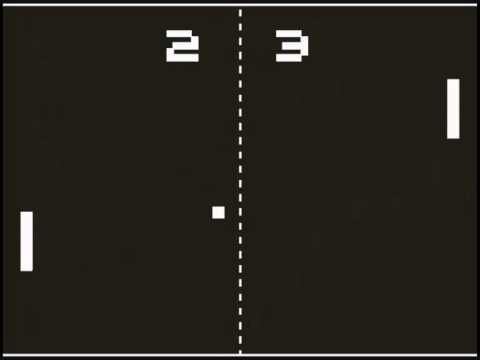
\includegraphics[width=0.5\textwidth]{obrazky-figures/pong.jpg}
    \caption{Hra pong 1972}
\end{figure}

\section{Popis problému a motivace}
V~rámci tohoto projektu jsem se setkal s~několika obtížemi.
Například příliš časté přerušení vyvolaného enkodéry, zákmity či problémový přístup ke sdílenémů zdroji. 
Překonáním těchto obtíží se stala hra poměrně plynulá a celkově hratelná.

\subsection{Technologické možnosti rotačních enkodérů} 
Rotační enkodér KY-040 je zařízení, které při otáčení osy poskytuje informace o~směru rotace a počtu otáček. 
Obsahuje také tlačítko, které se aktivuje stiskem osy. 
Na rozdíl od běžných potenciometrů umožňuje nekonečné otáčení v~obou směrech.
Pro zprovoznění tohoto enkodéru je potřeba propojit 5 pinů: CLK, DT, SW, + a GND.
V~kombinaci s~OLED displejem a ESP32 se z~enkodérů stává intuitivní ovládací prvek pro interaktivní aplikace.

\begin{figure}[H]
    \centering
    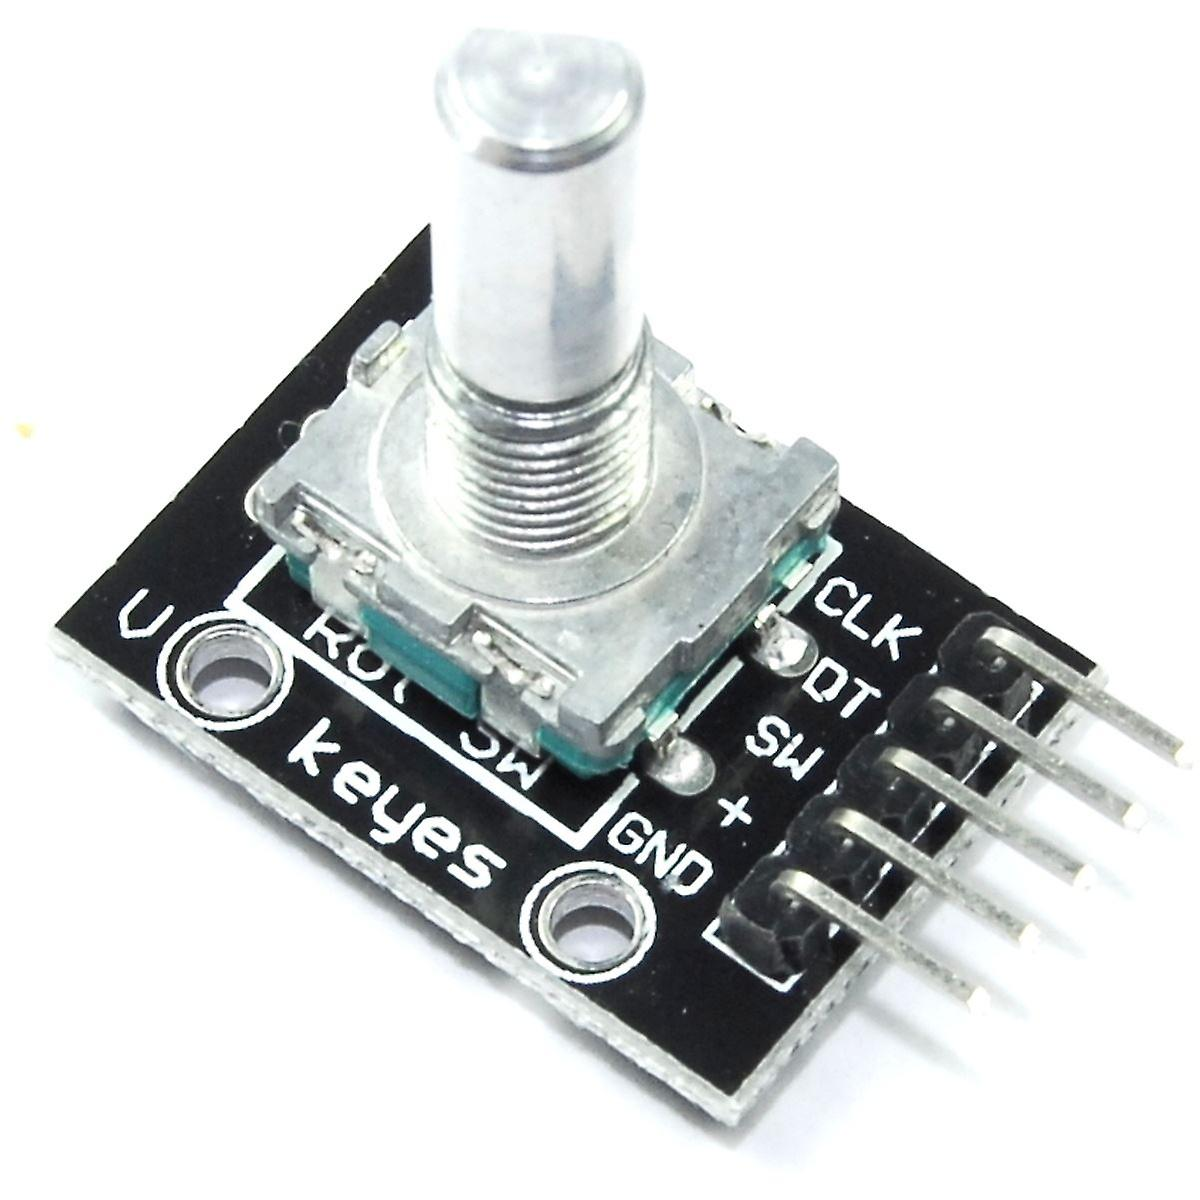
\includegraphics[width=0.5\textwidth]{obrazky-figures/enkoder.jpeg}
    \caption{enkodér KY-040}
\end{figure}

Mechanicky funguje tak, že enkodér generuje dva obdélníkové signály. 
Ty jsou fázově posunuté o~90°. 
Tyto signály odpovídají střídavému spínání kontaktů. 
Směr otáčení zjistíme podle fázového posunu a aktuální polohu určujeme podle počtu impulzů.\footnote{\url{https://embedded.fel.cvut.cz/sites/default/files/kurzy/lpe/rotary_encoder/Rotary_Encoder.pd}}

\begin{figure}[H]
    \centering
    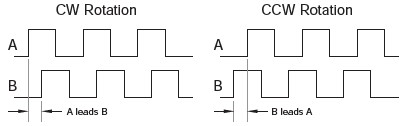
\includegraphics[width=0.75\textwidth]{obrazky-figures/graf_enkoder.jpg}
    \caption[Caption for LOF]{Graf fungování enkodéru\footnotemark}
\end{figure}
\footnotetext{\url{https://www.haydonkerkpittman.com/learningzone/whitepapers/incremental-encoder-signals}}

\subsection{Motivace k~výběru tématu}
Tento projekt jsem bral jako příležitost získat praktické zkušenosti s~integrací hardwarových komponent a softwarovým vývojem na mikrořadičích. 
Hra Pong je navíc aplikace, která kreativním způsobem využívá všechny komponenty uvedené v~zadání. 
Možnost pracovat po delší době s~hardwarem a zprovoznit na něm napodobeninu hry Pong bylo pro mě přínosné a přinejmenším zábavné. 

\section{Návrh řešení}
\subsection{Technologické prostředky}
\begin{itemize}
    \item \textbf{ESP32}
    \item \textbf{OLED displej}
    \item \textbf{Rotační enkodéry}
    \item \textbf{FreeRTOS}
\end{itemize}

\subsection{Funkční požadavky}
Aplikace by měla běžet plynule. 
Zobrazování by mělo být přesné a jednotlivé objekty by neměly zanechávat žádné chybné výstupy na displej.
Otáčení enkodérů by se mělo plynule a realisticky přenášet do hry.
Stisk tlačítka musí být správně zaznamenán a restartovat hru.

\subsection{Architektura řešení}
Pro správné zaznamenávání a přenášení dat do hry je použito přerušení pro enkodéry a tlačítka.
Každá hardwarová komponenta má vlastní proces, aby byl správně zaznamenáván a zpracováván v~reálném čase.
Míč je také realizován svým vlastním procesem, který zajišťuje plynulou aktualizaci jeho polohy.
Enkodéry mají fronty pro předávání událostí, které nastanou při přerušení.

\section{Implementace}
\subsection{Hardwarová konfigurace} \noindent
Rotační enkodéry a OLED displej jsou připojeny k~ESP32 následovně:
\begin{itemize}
    \item Zapojení enkodérů A~a B:\\ 
    \begin{verbatim}
        // Piny pro enkodery
        #define PLAYER_A_CLK GPIO_NUM_26
        #define PLAYER_A_DT  GPIO_NUM_25

        #define PLAYER_B_CLK GPIO_NUM_17
        #define PLAYER_B_DT  GPIO_NUM_16

        // Piny pro tlačítka
        #define PLAYER_A_BUTTON GPIO_NUM_13
        #define PLAYER_B_BUTTON GPIO_NUM_14
    \end{verbatim}
    \item Zapojení OLED displeje:\\
    \begin{verbatim}
        // Piny pro OLED display
        #define OLED_RST GPIO_NUM_27
        #define OLED_CS GPIO_NUM_5
        #define OLED_DC GPIO_NUM_4
        #define OLED_CLK GPIO_NUM_18
        #define OLED_MOSI GPIO_NUM_23
    \end{verbatim}
\end{itemize}

\subsection{Zpracování vstupů}
Pro zpracování signálů z~enkodérů a tlačítek byl použit systém přerušení.
V~následujícím kusu kódu je nastaveno, jaké změny na pinu aktivují přerušení, na kterých pinech bude nastaveno, definice pinů jako výstupních, použití pull-up rezistorů a přiřazení přerušení pro piny a funkci. 
\\ \\ \noindent
Nastavení přerušení:
\begin{verbatim}
    // Enkoder hráče A
    io_conf.intr_type = GPIO_INTR_ANYEDGE;
    io_conf.pin_bit_mask = (1ULL << PLAYER_A_CLK) | (1ULL << PLAYER_A_DT);
    io_conf.mode = GPIO_MODE_INPUT;
    io_conf.pull_up_en = GPIO_PULLUP_ENABLE;
    gpio_config(&io_conf);
    gpio_install_isr_service(0);
    gpio_isr_handler_add(PLAYER_A_CLK, player_a_isr_handler, NULL);
\end{verbatim}
\noindent
Obshluha přerušení:
\begin{verbatim}
    // Funkce pro přerušení enkoderu hráče A
    void IRAM_ATTR player_a_isr_handler(void* arg) {
        static int last_a = 0;
        int a = gpio_get_level(PLAYER_A_CLK);
        int b = gpio_get_level(PLAYER_A_DT);

        unsigned long interrupt_time = esp_timer_get_time() / 1000;

        if (a != last_a && a == 1 && 
            (interrupt_time - last_interrupt_time_a > DEBOUNCE_DELAY)) {
            BaseType_t xHigherPriorityTaskWoken = pdFALSE;
            int event = (b == a) ? 1 : -1; 
            xQueueSendFromISR(xQueueEncoderA,
                              &event, &xHigherPriorityTaskWoken);
            portYIELD_FROM_ISR(xHigherPriorityTaskWoken);
            last_interrupt_time_a = interrupt_time; 
        }
        last_a = a;
    }
\end{verbatim}

\subsection{Úlohy v~FreeRTOS} \noindent
Každý hráč má vlastní úlohu pro zpracování vstupů z~enkodérů.
\\ \\ \noindent
Pomocná úloha pro hráčský proces - zpracování fronty:
\begin{verbatim}
    // Pomocná funkce pro frontu hráče A
    void playerA_encoder_task(void *pvParameters) {
        int event;
        while (1) {
            if (xQueueReceive(xQueueEncoderA, &event, portMAX_DELAY)) {
                pos_y_player_a += event * 2;
                if (pos_y_player_a < 0) pos_y_player_a = 0;
                if (pos_y_player_a > 52) pos_y_player_a = 52;
                update_player_a_flag = true;
            }
        }
    }
\end{verbatim}
\noindent
Úloha pro hráčský proces - volání funkce pro aktualizace pozice hráče A:
\begin{verbatim}
    // Funcke pro proces hráč A
    void playerA_task(void *pvParameters) {
        while (1) {
            if (update_player_a_flag) {
                update_player_a();
                update_player_a_flag = false;
            }
            delay(pdMS_TO_TICKS(10));
        }
    }
\end{verbatim}
\noindent
Míč má také vlastní úlohu pro aktualizaci jeho polohy:
\begin{verbatim}
    // Funkce pro proces míč
    void ball_task(void *pvParameters) {
        while (1) {
            // Rychlost míče
            if (time % speed == 0) {
                ball_pos_x += ball_x_dir;
                ball_pos_y += ball_y_dir;
            }

            // Kontrola hranic displaye osy X
            if (ball_pos_x < 3) {
                ball_x_dir = -ball_x_dir;
                ball_pos_x = 3;
                if (!(ball_pos_y >= pos_y_player_b - 2 && 
                    ball_pos_y <= pos_y_player_b + 10)) {
                    game = 0;
                }
            } else if (ball_pos_x > 122) {
                ball_x_dir = -ball_x_dir;
                ball_pos_x = 122;
                if (!(ball_pos_y >= pos_y_player_a - 2 && 
                ball_pos_y <= pos_y_player_a + 10)) {
                    game = 0;
                }
            }

            // Kontrola hranic displaye osy Y
            if (ball_pos_y < 0) {
                ball_y_dir = -ball_y_dir;
                ball_pos_y = 0;
            } else if (ball_pos_y > 61) {
                ball_y_dir = -ball_y_dir;
                ball_pos_y = 61;
            }

            // Vykreslení míče
            if (xSemaphoreTake(xBallSemaphore, portMAX_DELAY) == pdTRUE) {
                update_ball();
                xSemaphoreGive(xBallSemaphore);
            }
            delay(DELAY);
        }
    }
\end{verbatim}

\subsection{Zobrazení na OLED displeji}
Hráčské plošiny jsou vykreslovány na základě metody přerušení aktivované pohybem enkodérů.
Míč je samostatný proces, který žádá o~vykreslení periodicky.
Kvůli využití jednoho sdíleného zdroje (OLED displeje) je využit semafor.
Proces míče má tedy nastavenou vyšší prioritu a měl by mít přednost při přístupu k~displeji.
\\ \\ \noindent
Aktualizace hráčské pozice na displeji:
\begin{verbatim}
    // Vykreslení pozice hráče A
    void update_player_a() {
        if (xSemaphoreTake(xBallSemaphore, portMAX_DELAY) == pdTRUE) {
            for (int i = pos_x_player_a; i < 128; i++) {
                for (int j = 0; j < 63; j++) {
                    if (j >= pos_y_player_a && j <= pos_y_player_a + 10) {
                        set_pixel(i, j, 1);
                    } else {
                        set_pixel(i, j, 0);
                    } 
                }
            }
            xSemaphoreGive(xBallSemaphore);
        }
    }
\end{verbatim}

Aktualizace míče na displeji:
\begin{verbatim}
    // Vykreslení pozice míče
    void update_ball() {
        for (int i = 0; i < 3; i++) {
            for (int j = 0; j < 3; j++) {
                if(prev_ball_pos_x + i != 63){
                    set_pixel(prev_ball_pos_x + i, prev_ball_pos_y + j, 0);
                    set_pixel(ball_pos_x + i, ball_pos_y + j, 1);
                }
            }
        }
        prev_ball_pos_x = ball_pos_x;
        prev_ball_pos_y = ball_pos_y;
    }
\end{verbatim}


\section{Testování, výsledky a autoevaluace}
Testování proběhlo poměrně primitivně. Pustupným upravováním jednotlivých delayů a opětovným testováním bylo potřeba zajistit plynulost a celkový kladný dojem ze hry.

\subsection{Výsledky}
Přestože jsem využil všechny mnou známé prostředky k~řešení problému s~jedním sdíleným zdrojem se mi nepodařilo najít stoprocentně plynulé a bezproblémové řešení.
Myslím si ale, že jsem se k~tomu velmi přiblížil a hra celkové působí dobrým dojmem.

\subsection{autoevaluace}
Pozitiva řešení:
\begin{itemize}
    \item{Dle mého vlastního názoru je řešení komplexní a je řešeno nadmíru původního zadání.}
    \item{Byly splněny povinné i nepovinné body zadání.}
    \item{Byly použity další komponenty nedefinované zadáním, konkrétě OLED dispej.}
    \item{Také byly použity technologie nedefinované zadáním a to vuyžití více procesů díky FreeRTOS, využití front a semaforu.}
\end{itemize}

Nedostatky:
\begin{itemize}
    \item{Kompromis požadavků na sdílený zdroj (hráči a míčem) při rychlém pohybu hráčů způsobil, že míč je nepatrně zpomalen.}
    \item{Dokumentace není tak detailní a komplexní, jak bych si přál.}
\end{itemize}

Hodnocení v rámci projektu:
\begin{itemize}
    \item{E - 2b}
    \item{F - 4,5b}
    \item{Q - 2b}
    \item{P - 0-2b}
    \item{D - 2,5b}
\end{itemize}

Dle tabulky hodnocení uvedené v zadání a pomocí vzorečku na celkový počet bodů bych tento projekt ohodnotil 10 až 12 body v závislosti na prezentaci.

\section{Závěr}
Pomocí mikrořadiče ESP32, dvojice rotačních enkodérů s~tlačítky KX/Y-040 a OLED displeje jsem vytvořil funkční napodobeninu hry Pong.
Jak otáčení os enkodérů, tak mačkání tlačítek bylo realizováno pomocí přerušení. 
Pro lepší synchronizaci a plynulost hry byly využity fronty, semafor a procesy pro jednotlivé úkoly.
Hra je hratelná a poměrně plynulá.
Tento projekt splňuje všechny povinné i volitelné body zadání.

\end{document}
